\begin{document}

\title {\ZHH \huge 雪崩与过载保护}
\author {\small gaccob}
\date {\small 2013 年 1 月 28 日}
\maketitle

\section {\ZHH 什么是“雪崩”? } {
    { 这里的"雪崩"是一种形象的比喻, 是指在后台的集群服务中, 由于某一个点不可用(硬件故障, 超出负载能力等), 而扩散到整个集群, 导致整个集群无法服务. } \par
    { 其根本原因, 在于后台的服务单元, 没有做好过载情况下的保护, 在超出自己负载能力的情况下无法正常提供服务, 而这一行为又反过来加剧了整个系统的负载, 从而使得整个服务迅速崩溃, 不可用. } \par
}

\gaccobsplitinv

\section {\ZHH 一则案例} {
    { 这则雪崩案例来自腾讯大讲堂, 原文链接\href{http://djt.qq.com/article/view/156}{在这里} } \par
    \begin {figure}[htbp]
        \centering
        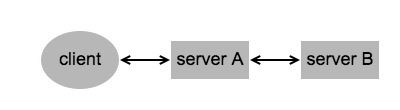
\includegraphics [width=300pt, keepaspectratio] {case.jpg}
    \end {figure}
    \begin{itemize}
        \item { client通过udp访问Server A, 超时为1s, 正常峰值在30次请求/秒.  Server A 以同步的方式访问 Server B, 超时100ms,  Server B 的处理速度在20ms左右, 相当于每秒能响应50次请求; }
        \item { 某一天系统更新后,  Server B 的相应能力降到20次/秒, Server A 的峰值请求超出了 Server B 的负载, 发生了大量失败, 而失败的用户往往特别喜欢重试, 当这些重试的请求到达 Server B 时,进一步加剧了负载, 从而导致整个网络服务不可用, 雪崩. }
        \item { 根本的原因在于:  Server B 给出的同步超时在100ms, 说明了 Server B 的承诺的负载能力在10次/s, 当 Server A 的请求超过这个值时, 就有过载的风险. 在系统更新之前没有发生, 只是被掩盖了而已. }
    \end{itemize}
}

\gaccobsplitinv

\section {\ZHH 怎么防止雪崩} {
    {结合上面的案例, 来看看应该怎么做过载保护, 防止雪崩. }
    \begin{itemize}
    \item {从\textcolor{blue}{架构}上说, 每一个server最好都设计成可分布式服务的, 厚重的服务按照功能, 优先级, 处理速度拆分, 保证具备扩容能力. 一旦某一点成为了单点, 就有可能成为负载瓶颈, 有过载的风险. 如果案例中的 Server B 在业务请求量上来时, 可以迅速通过增加 Server B 的进程数扩容, 也许就能避免这一场雪崩事故. }
    \item {从\textcolor{blue}{监控}上说, 后台的server的监控要到位, 迅速的扩容响应离不开全方位的监控告警机制. 监控最好能精细到进程粒度, cpu, 内存, 网络流量, 磁盘IO, 都要设置阈值告警, 一旦有过载的苗头, 先加机器加资源保护住再来看问题. }
    \item {从\textcolor{blue}{保护}上说, 第一步是保护后端, 整个系统中的每一个点, 都应该清楚的知道自己后端服务的承载能力, 例如这里 Server B 的承载能力是10次/秒,  Server A 应该保证到后端 Server B 的业务请求量低于这个值, 超过了应该拒绝; 另外, 客户端也很重要, 要做好失败后的重试保护, 坚决不能让用户频繁的发起重试请求; 第二步是自我保护, 一个有效的手段是超时机制, 每一个业务, 在收到请求之后, 如果发现已经超过预设的时间就直接拒绝 (通信协议中需要带时间戳), 不再增加无谓的压力, 防止问题扩散;}
    \item {从\textcolor{blue}{流程}上说, 在每一次新功能的发布中, 如果能做灰度就尽量做, 实在做不了也最好在开发环境上做好演习测试. 对于服务器来说, 稳定是首要大事, 特别是在重大版本更新之际, 小心驶的万年船. (最不赞同的, 是在没有经过完善的, 逐步的测试, 就一下子大批量放号, 这是对整个项目整个团队的不负责)}
    \end{itemize}
}

\end{document}
